\documentclass[11pt]{article}
\usepackage[margin=0.9in]{geometry}
\usepackage{times}
\usepackage{xcolor}
\usepackage{tikz}
\usetikzlibrary{arrows.meta,positioning,shapes.geometric,backgrounds}
\usepackage{enumitem}
\usepackage{titlesec}
\usepackage{tcolorbox}

\definecolor{ink}{HTML}{1a1a1a}
\definecolor{blue}{HTML}{2a78d6}
\definecolor{orange}{HTML}{eb6834}
\definecolor{green}{HTML}{1baf7a}
\definecolor{grayb}{HTML}{f2f2f0}
\definecolor{grayl}{HTML}{d8d7d0}

\titleformat{\section}{\large\bfseries\color{blue}}{}{0em}{}
\titlespacing{\section}{0pt}{10pt}{4pt}
\setlength{\parindent}{0pt}
\setlength{\parskip}{5pt}

% Analogy callout box
\newtcolorbox{analogy}{colback=grayb,colframe=orange,boxrule=0.8pt,
  left=8pt,right=8pt,top=5pt,bottom=5pt,arc=3pt,
  fontupper=\normalsize}

\begin{document}

\begin{center}
{\LARGE\bfseries\color{ink} How Our Project Works}\\[2pt]
{\large A Simple, No-Jargon Explanation}\\[4pt]
{\small\itshape A Multi-Protocol Cyber-Deception Framework with AI and Blockchain}
\end{center}

\hrule
\vspace{6pt}

\section*{\color{blue}The Big Idea in One Sentence}

We build \textbf{fake computer systems that look real to hackers}. When a hacker
attacks one, we secretly \textbf{watch everything they do}, use \textbf{AI to
reply convincingly} so they keep going, and \textbf{lock the evidence in a
tamper-proof record} nobody can secretly change.

\begin{analogy}
\textbf{Real-life comparison --- the fake shop.} Imagine a shop owner tired of
shoplifters. So they open a \emph{decoy shop} full of fake goods, with hidden
cameras everywhere. Thieves walk in thinking it's real, and every move they make
is recorded --- but nothing valuable is ever at risk. \textbf{Our project is
that decoy shop, but for computers.}
\end{analogy}

\section*{\color{blue}Why Do We Need This?}

Normal ``traps'' for hackers (called \emph{honeypots}) have a weakness: they give
the \emph{same fixed answers} every time. A smart hacker quickly notices the
answers are robotic and realises ``this is a trap!'' and leaves. It's like a
mannequin in a shop --- stand near it for a second and you know it isn't a real
person.

\textbf{We fix this with three upgrades:}

\vspace{4pt}
% ---- Three pillars diagram ----
\begin{center}
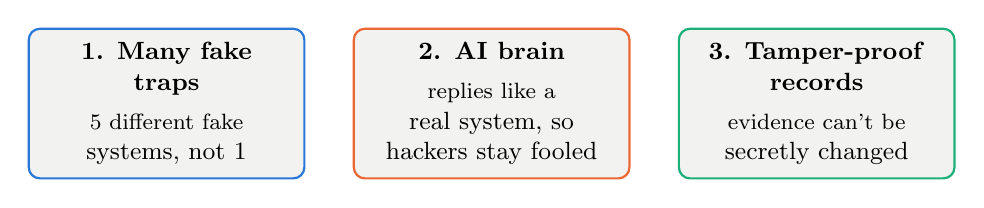
\begin{tikzpicture}[font=\small,node distance=6mm]
\tikzstyle{pill}=[draw,rounded corners=4pt,minimum width=3.5cm,minimum height=1.9cm,
  align=center,thick,fill=grayb]
\node[pill,draw=blue]   (a) {\textbf{1. Many fake}\\\textbf{traps}\\[3pt]\footnotesize 5 different fake\\systems, not 1};
\node[pill,draw=orange,right=of a] (b) {\textbf{2. AI brain}\\[3pt]\footnotesize replies like a\\real system, so\\hackers stay fooled};
\node[pill,draw=green,right=of b]  (c) {\textbf{3. Tamper-proof}\\\textbf{records}\\[3pt]\footnotesize evidence can't be\\secretly changed};
\end{tikzpicture}
\end{center}

\section*{\color{blue}Upgrade 1: Many Fake Traps (not just one)}

Instead of one fake system, we run \textbf{five} --- each pretending to be a
different thing a company owns: a login server, a database, an AI service, a
crypto wallet system, and a software-build server. This catches many kinds of
attackers at once.

\begin{analogy}
\textbf{Comparison --- a house with decoy valuables in every room.} Instead of
one fake safe, you place a fake jewellery box in the bedroom, a fake wallet in
the hall, a fake laptop in the study. Whichever room a burglar enters, a camera
is already watching.
\end{analogy}

\section*{\color{blue}Upgrade 2: The AI Brain (the clever part)}

When a hacker types something we've never seen before, older traps freeze or give
a wrong answer --- an instant giveaway. Instead, we ask an \textbf{AI (a language
model)} to \emph{make up a realistic reply on the spot}, exactly like a real
computer would. The hacker never realises they're talking to a decoy.

\begin{analogy}
\textbf{Comparison --- a fake receptionist who never breaks character.} A cardboard
cut-out receptionist fools no one. But a trained actor who answers any question
naturally? You'd believe they're real. \textbf{The AI is that actor.}
\end{analogy}

To keep it fast \emph{and} smart, we use a \textbf{3-step shortcut}: common
questions get instant pre-written answers; repeated questions are remembered; only
brand-new questions go to the (slower) AI. Best of both worlds.

\vspace{4pt}
\begin{center}
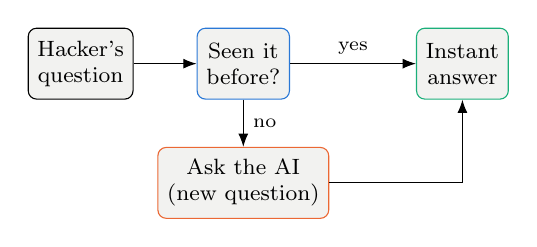
\begin{tikzpicture}[font=\footnotesize,node distance=8mm,>=Latex]
\tikzstyle{b}=[draw,rounded corners=3pt,minimum height=0.9cm,align=center,fill=grayb]
\node[b] (q) {Hacker's\\question};
\node[b,right=of q,draw=blue] (s) {Seen it\\before?};
\node[b,right=1.6cm of s,draw=green] (f) {Instant\\answer};
\node[b,below=6mm of s,draw=orange] (ai) {Ask the AI\\(new question)};
\draw[->] (q)--(s);
\draw[->] (s)--node[above,font=\scriptsize]{yes}(f);
\draw[->] (s)--node[right,font=\scriptsize]{no}(ai);
\draw[->] (ai) -| (f);
\end{tikzpicture}
\end{center}

\section*{\color{blue}Upgrade 3: Tamper-Proof Records (blockchain)}

Every action the hacker takes is recorded. But there's a catch: since the trap is
being attacked, a clever hacker might try to \emph{delete or edit} the record of
what they did. So we take a unique ``fingerprint'' of each record and lock that
fingerprint into a \textbf{blockchain} --- a record that, once written, can never
be secretly changed.

\begin{analogy}
\textbf{Comparison --- a notary stamp / wax seal.} Think of an important letter
sealed with wax. If anyone opens or alters it, the seal breaks and everyone can
see it was tampered with. Our system does this digitally: if even one letter of
a record is changed later, the ``fingerprint'' no longer matches, and the
tampering is caught instantly.
\end{analogy}

\newpage

\section*{\color{blue}The Whole Story: One Attack, Start to Finish}

Here is what happens, step by step, when a hacker attacks our system:

\vspace{6pt}
\begin{center}
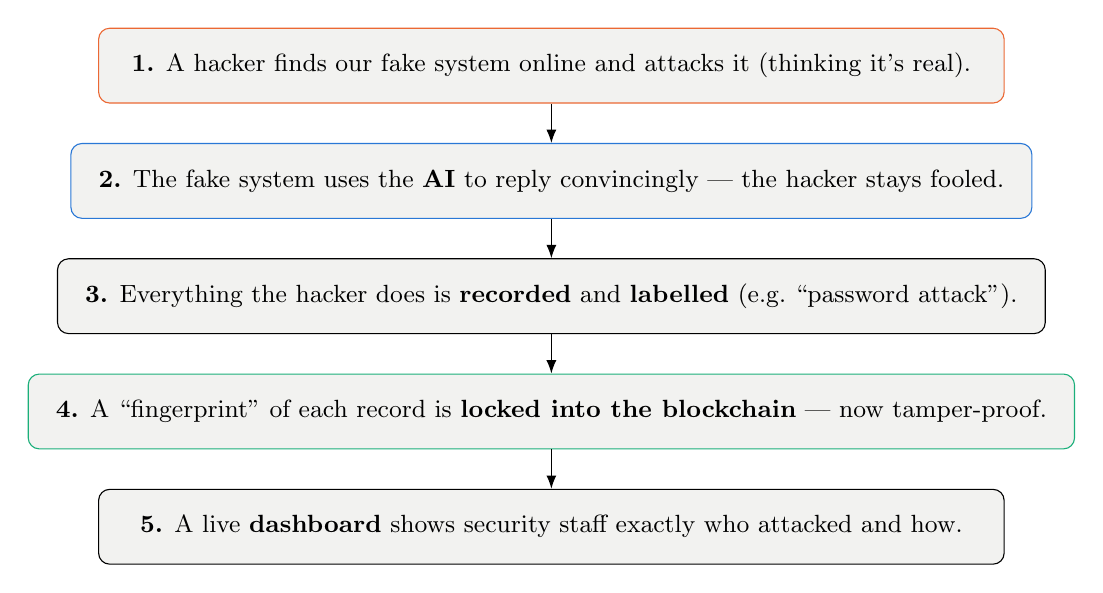
\begin{tikzpicture}[font=\small,>=Latex,node distance=5mm]
\tikzstyle{s}=[draw,rounded corners=4pt,minimum width=11.5cm,minimum height=0.95cm,
  align=left,fill=grayb,inner xsep=10pt]
\node[s,draw=orange] (1) {\textbf{1.} A hacker finds our fake system online and attacks it (thinking it's real).};
\node[s,draw=blue,below=of 1] (2) {\textbf{2.} The fake system uses the \textbf{AI} to reply convincingly --- the hacker stays fooled.};
\node[s,below=of 2] (3) {\textbf{3.} Everything the hacker does is \textbf{recorded} and \textbf{labelled} (e.g.\ ``password attack'').};
\node[s,draw=green,below=of 3] (4) {\textbf{4.} A ``fingerprint'' of each record is \textbf{locked into the blockchain} --- now tamper-proof.};
\node[s,below=of 4] (5) {\textbf{5.} A live \textbf{dashboard} shows security staff exactly who attacked and how.};
\draw[->] (1)--(2); \draw[->] (2)--(3); \draw[->] (3)--(4); \draw[->] (4)--(5);
\end{tikzpicture}
\end{center}

\vspace{4pt}

\section*{\color{blue}What Makes Ours Special}

Most existing hacker-traps do only \emph{one} of these things. Ours is the first
to combine \textbf{all three} --- many fake systems + a convincing AI brain +
tamper-proof evidence --- in a single package.

\begin{center}
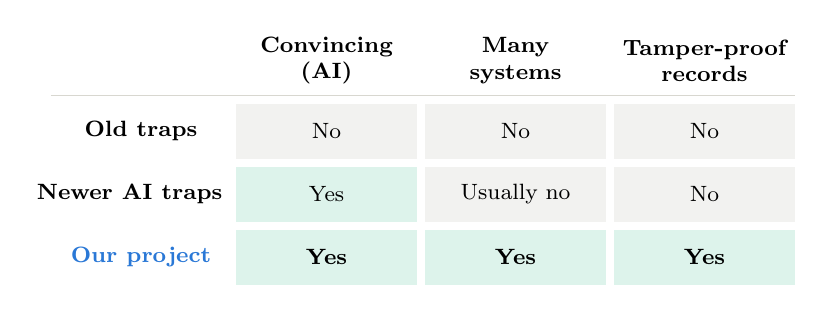
\begin{tikzpicture}[font=\footnotesize]
\tikzstyle{h}=[font=\bfseries\footnotesize]
\tikzstyle{cell}=[minimum width=2.3cm,minimum height=0.7cm,align=center]
\tikzstyle{yes}=[cell,fill=green!15]
\tikzstyle{no}=[cell,fill=grayb]
% headers
\node[cell,h] at (0,0) {};
\node[cell,h] at (2.4,0) {Convincing\\(AI)};
\node[cell,h] at (4.8,0) {Many\\systems};
\node[cell,h] at (7.2,0) {Tamper-proof\\records};
% row: old traps
\node[cell,h,anchor=east] at (1.2,-0.9) {Old traps};
\node[no] at (2.4,-0.9) {No};
\node[no] at (4.8,-0.9) {No};
\node[no] at (7.2,-0.9) {No};
% row: AI-only traps
\node[cell,h,anchor=east] at (1.2,-1.7) {Newer AI traps};
\node[yes] at (2.4,-1.7) {Yes};
\node[no] at (4.8,-1.7) {Usually no};
\node[no] at (7.2,-1.7) {No};
% row: ours
\node[cell,h,anchor=east] at (1.2,-2.5) {\color{blue}Our project};
\node[yes] at (2.4,-2.5) {\textbf{Yes}};
\node[yes] at (4.8,-2.5) {\textbf{Yes}};
\node[yes] at (7.2,-2.5) {\textbf{Yes}};
\draw[grayl] (-1.1,-0.45) -- (8.35,-0.45);
\end{tikzpicture}
\end{center}

\vspace{6pt}

\section*{\color{blue}The One-Line Summary (for a viva)}

\begin{tcolorbox}[colback=blue!6,colframe=blue,boxrule=1pt,arc=3pt]
\textit{``We built five fake computer systems that use AI to convincingly fool
attackers into revealing their methods, and we lock every piece of evidence into
a blockchain so it can never be secretly tampered with --- giving us honest,
trustworthy intelligence about how real attacks happen.''}
\end{tcolorbox}

\vspace{4pt}
\begin{center}
\footnotesize\color{ink!70}
Real terms (so you can connect the simple idea to the technical words):\\
Fake trap = \textbf{honeypot} \quad|\quad AI brain = \textbf{large language model (LLM)}
\quad|\quad Fingerprint = \textbf{SHA-256 hash} \quad|\quad Tamper-proof record = \textbf{blockchain}
\end{center}

\end{document}
